We can use SAT for many purposes, like validation, satisfiability of properties but also for Constraint Optimization Problems.
\begin{example}
    e.g. Optimal map colouring. \vspace{7pt}

    Can we assign a color to the regions such that adjacent regions have different colors? \vspace{3.5pt}
    \begin{center}
        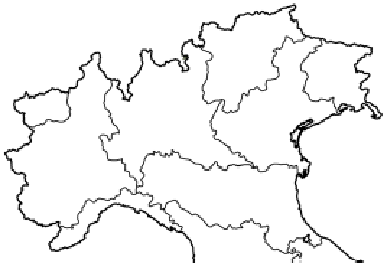
\includegraphics[width = 0.3\textwidth]{img/img4.png}
    \end{center} \vspace{3.5pt}
    
    \textbf{Boolean decision variables}. \\ 
    A boolean decision variable $x_{ic}$ describes each possible color $c \in \{1, \dots, k\}$ and region $v_i \in V$. 
    \begin{itemize}
        \renewcommand{\labelitemi}{-}
        \item $x_{ic} = T$ means that a region $v_i$ is assigned to the color $c$.
    \end{itemize} \vspace{7pt}

    \textbf{Constraints}.
    \begin{itemize}
        \renewcommand{\labelitemi}{-}
        \item Each region gets at least one color.
        $$ \forall v_i \in V, x_{i1} \vee \dots \vee x_{ik} $$
        More synthetically:
        $$ \forall v_i \in V, \bigvee_{1 \leq v \leq k} x_{ic} $$
        This new expression tells us the same thing as the original one, we can assume that between all the boolean decision variables $x_{ic}$ we have a 
        logical \textit{OR}. 
        \item Neighboring regions takes different colors.
        $$ \forall (v_i, v_j) \in E, \forall c \in \{1, \dots, k\}, \neg (x_{ic} \wedge x_{jc}) $$
        Or more synthetically:
        $$ \forall (v_i, v_j) \in E, \bigwedge_{1 \leq c \leq k} \neg (x_{ic} \wedge x_{jc}) $$
        For each pair of neighboring regions, they cannot share the same color.
    \end{itemize}
\end{example}